%File: anonymous-submission-latex-2023.tex
\documentclass[letterpaper]{article} % DO NOT CHANGE THIS
\usepackage[submission]{aaai23}  % DO NOT CHANGE THIS
\usepackage{times}  % DO NOT CHANGE THIS
\usepackage{helvet}  % DO NOT CHANGE THIS
\usepackage{courier}  % DO NOT CHANGE THIS
\usepackage[hyphens]{url}  % DO NOT CHANGE THIS
\usepackage{graphicx} % DO NOT CHANGE THIS
\urlstyle{rm} % DO NOT CHANGE THIS
\def\UrlFont{\rm}  % DO NOT CHANGE THIS
\usepackage{natbib}  % DO NOT CHANGE THIS AND DO NOT ADD ANY OPTIONS TO IT
\usepackage{caption} % DO NOT CHANGE THIS AND DO NOT ADD ANY OPTIONS TO IT
\frenchspacing  % DO NOT CHANGE THIS
\setlength{\pdfpagewidth}{8.5in} % DO NOT CHANGE THIS
\setlength{\pdfpageheight}{11in} % DO NOT CHANGE THIS
%
% These are recommended to typeset algorithms but not required. See the subsubsection on algorithms. Remove them if you don't have algorithms in your paper.
\usepackage{algorithm}
\usepackage{algorithmic}

\usepackage{amsmath,amssymb,amsfonts}
\usepackage{graphicx}
\usepackage{textcomp}
\usepackage{xcolor}
\usepackage{booktabs}
\usepackage{stmaryrd}
% \usepackage{algorithmicx}
\usepackage{framed}
\usepackage{enumitem}
% \usepackage[ruled]{algorithm2e}
\usepackage{multirow}
\usepackage{arydshln}
\usepackage{subfigure} % 子图包



%
% These are are recommended to typeset listings but not required. See the subsubsection on listing. Remove this block if you don't have listings in your paper.
\usepackage{newfloat}
\usepackage{listings}
\DeclareCaptionStyle{ruled}{labelfont=normalfont,labelsep=colon,strut=off} % DO NOT CHANGE THIS
\lstset{%
	basicstyle={\footnotesize\ttfamily},% footnotesize acceptable for monospace
	numbers=left,numberstyle=\footnotesize,xleftmargin=2em,% show line numbers, remove this entire line if you don't want the numbers.
	aboveskip=0pt,belowskip=0pt,%
	showstringspaces=false,tabsize=2,breaklines=true}
\floatstyle{ruled}
\newfloat{listing}{tb}{lst}{}
\floatname{listing}{Listing}
%
% Keep the \pdfinfo as shown here. There's no need
% for you to add the /Title and /Author tags.
\pdfinfo{
/TemplateVersion (2023.1)
}

% DISALLOWED PACKAGES
% \usepackage{authblk} -- This package is specifically forbidden
% \usepackage{balance} -- This package is specifically forbidden
% \usepackage{color (if used in text)
% \usepackage{CJK} -- This package is specifically forbidden
% \usepackage{float} -- This package is specifically forbidden
% \usepackage{flushend} -- This package is specifically forbidden
% \usepackage{fontenc} -- This package is specifically forbidden
% \usepackage{fullpage} -- This package is specifically forbidden
% \usepackage{geometry} -- This package is specifically forbidden
% \usepackage{grffile} -- This package is specifically forbidden
% \usepackage{hyperref} -- This package is specifically forbidden
% \usepackage{navigator} -- This package is specifically forbidden
% (or any other package that embeds links such as navigator or hyperref)
% \indentfirst} -- This package is specifically forbidden
% \layout} -- This package is specifically forbidden
% \multicol} -- This package is specifically forbidden
% \nameref} -- This package is specifically forbidden
% \usepackage{savetrees} -- This package is specifically forbidden
% \usepackage{setspace} -- This package is specifically forbidden
% \usepackage{stfloats} -- This package is specifically forbidden
% \usepackage{tabu} -- This package is specifically forbidden
% \usepackage{titlesec} -- This package is specifically forbidden
% \usepackage{tocbibind} -- This package is specifically forbidden
% \usepackage{ulem} -- This package is specifically forbidden
% \usepackage{wrapfig} -- This package is specifically forbidden
% DISALLOWED COMMANDS
% \nocopyright -- Your paper will not be published if you use this command
% \addtolength -- This command may not be used
% \balance -- This command may not be used
% \baselinestretch -- Your paper will not be published if you use this command
% \clearpage -- No page breaks of any kind may be used for the final version of your paper
% \columnsep -- This command may not be used
% \newpage -- No page breaks of any kind may be used for the final version of your paper
% \pagebreak -- No page breaks of any kind may be used for the final version of your paperr
% \pagestyle -- This command may not be used
% \tiny -- This is not an acceptable font size.
% \vspace{- -- No negative value may be used in proximity of a caption, figure, table, section, subsection, subsubsection, or reference
% \vskip{- -- No negative value may be used to alter spacing above or below a caption, figure, table, section, subsection, subsubsection, or reference

\setcounter{secnumdepth}{0} %May be changed to 1 or 2 if section numbers are desired.

% The file aaai23.sty is the style file for AAAI Press
% proceedings, working notes, and technical reports.
%

% Title

% Your title must be in mixed case, not sentence case.
% That means all verbs (including short verbs like be, is, using,and go),
% nouns, adverbs, adjectives should be capitalized, including both words in hyphenated terms, while
% articles, conjunctions, and prepositions are lower case unless they
% directly follow a colon or long dash
\title{2PC-NNP: Two-Party Computation Framework for Neural Network Predictions \\ Via a Novel Secret Comparison protocol}
\author{
    %Authors
    % All authors must be in the same font size and format.
    Written by AAAI Press Staff\textsuperscript{\rm 1}\thanks{With help from the AAAI Publications Committee.}\\
    AAAI Style Contributions by Pater Patel Schneider,
    Sunil Issar,\\
    J. Scott Penberthy,
    George Ferguson,
    Hans Guesgen,
    Francisco Cruz\equalcontrib,
    Marc Pujol-Gonzalez\equalcontrib
}
\affiliations{
    %Afiliations
    \textsuperscript{\rm 1}Association for the Advancement of Artificial Intelligence\\
    % If you have multiple authors and multiple affiliations
    % use superscripts in text and roman font to identify them.
    % For example,

    % Sunil Issar, \textsuperscript{\rm 2}
    % J. Scott Penberthy, \textsuperscript{\rm 3}
    % George Ferguson,\textsuperscript{\rm 4}
    % Hans Guesgen, \textsuperscript{\rm 5}.
    % Note that the comma should be placed BEFORE the superscript for optimum readability

    1900 Embarcadero Road, Suite 101\\
    Palo Alto, California 94303-3310 USA\\
    % email address must be in roman text type, not monospace or sans serif
    publications23@aaai.org
%
% See more examples next
}

%Example, Single Author, ->> remove \iffalse,\fi and place them surrounding AAAI title to use it
\iffalse
\title{My Publication Title --- Single Author}
\author {
    Author Name
}
\affiliations{
    Affiliation\\
    Affiliation Line 2\\
    name@example.com
}
\fi

\iffalse
%Example, Multiple Authors, ->> remove \iffalse,\fi and place them surrounding AAAI title to use it
\title{My Publication Title --- Multiple Authors}
\author {
    % Authors
    First Author Name,\textsuperscript{\rm 1}
    Second Author Name, \textsuperscript{\rm 2}
    Third Author Name \textsuperscript{\rm 1}
}
\affiliations {
    % Affiliations
    \textsuperscript{\rm 1} Affiliation 1\\
    \textsuperscript{\rm 2} Affiliation 2\\
    firstAuthor@affiliation1.com, secondAuthor@affilation2.com, thirdAuthor@affiliation1.com
}
\fi


% REMOVE THIS: bibentry
% This is only needed to show inline citations in the guidelines document. You should not need it and can safely delete it.
\usepackage{bibentry}
% END REMOVE bibentry

\begin{document}

\maketitle

\begin{abstract}

    Deep learning has achieved overwhelming successes in many fields, including image classification, speech recognition, machine translation etc.
    % These successes are largely due to the availability of big data and compute power.
    A pre-trained deep neural network model can predict the outcomes
    for a given data point. Such a deep neural network model can be served by
    specialized AI companies to users as a cloud prediction services.
    However, such a service model faces a privacy dilemma: neither AI companies nor
    users want to expose their private information.
    To achieve both model privacy and input data privacy,
    secure multi-party computation can utilized to evaluate prediction outcomes. However,
    this strategy is further complicated due to the complex deep learning prediction process.
    Currently, all existing solutions are very inefficient for employing complex asymmetric cryptographic operations.

    We propose 2PC-NNP, a two-party computation (2PC) framework for efficient neural network predictions.
    2PC-NNP is highly efficient because it does not use any asymmetric cryptography to simultaneously preserve model privacy and input data privacy.
    The core of 2PC-NNP is a novel and efficient two-party comparison protocol,
    which consits of three rounds of interactions without any oblivious transfer.
    From this building block, we construct the complete scheme for evaluating layers of the neural network, including the convolution layer, the pooling layer and the ReLu function.
		We formally prove that 2PC-NNP is {\bf secure} and also fully implement it with Python.
    Comprehensive experiments show that 2PC-NNP on resnet50
    costs only 23.86 seconds in computation and 100.13 seconds in communication.

    % We tested with the resnet50 network,
    % and one prediction only required 23.86 seconds of computation time and 100.13 seconds of communication time.
    % 我们设计了2PC-NNP来高效地计算这个问题。相比之前的工作,2PC-NNP基于一种新的比较协议,不需要使用OT协议和混淆电路,
    % 仅仅需要三次交互即可计算得到隐私输入的符号。我们在此基础上设计了计算神经网络各个层的方法。我们使用resnet50网络进行了测试,
    % 一次预测仅需要23.86秒的计算时间和100.13秒的通讯时间。


\end{abstract}


\section{Introduction}



    \noindent Deep learning, a popular research direction in the field of machine learning,
    has brought major breakthroughs to computer vision, speech recognition, natural language process, machine translation, etc. Recently, deep learning also made significant progress in bioinformatics, drug discovery and material sciences. A deep neural network model is obtained by training on
		a given training data set, which requires a large amount of training data and sufficient compute power.
		After the training step, the resultant deep neural network model is used to predict
		outcomes for a given data point. It is important to protect both the training phase and the predicting phase, while this work mainly focus on the prediction phase.

    % The application of neural network consists of two stages:
    % (1) training stage: the model is trained with training data,
    % (2) prediction stage: the pre-trained model is used to classify the input data.
    % This work mainly focus on the prediction stage.

    Machine learning as a service (MLaaS) is a range of machine learning tools offered by cloud service providers \cite{ChironCloud}.
    Some tasks that cannot be easily accomplished by data owner can be outsourced to
    the companies who provide cloud-based pre-trained deep learning model.
    For example, the CT images of lungs taken by hospitals
    can be transferred to the cloud computing center
    supported by major technical companies for medical diagnosis.
    However, during this period, the data owner inevitably reveals his input images,
    leading to a privacy leakage.

    To address this issue, privacy preserving machine learning based on secure multi-party
    computation (MPC) is proposed.
    MPC computation protocol enables players to evaluate a public function
    with multiple private secret inputs from different players.
    It provides the value of the public function or the shares of the value with each player
    without disclosing more information than what can be inferred from the result.
    Via performing MPC protocols,
    multiple parties can evaluate the prediction without disclosing the input image.
    The two parties computation (2PC) setting which only involves two parties is a particular case of MPC
    and the 2PC setting is used throughout the paper.

    The biggest difficulty of 2PC framework is that it costs too much to
    evaluate the comparison operation.
    The previous works usually utilize the asymmetric encryption
    operations like the  OT protocol and the garbled circuit,
    leading to large time cost.


    \subsection{Our contributions and overview}%%%%%%%%%%%%%%%%%%%%%%%%%%%%%%%%%%%%%%%%%%%%%%%%%%%%%%%%%%%%%%%%%%%%%%%%%%%%%%%%%%%%%%%%%%%%%%%%%%%%
    Here we summarize our contributions on a very high level.


    \begin{itemize}
        \item \textbf{2PC-comparison protocol}.
        We begin with the building block of our work, a brand new 2PC-$\mathtt{comparison}$ protocol,
        which does not require the asymmetric cryptography operations or the bit-level operations
        and only needs three rounds of interactions to calculate the sign of the secret input.
        The speed of it is 40$\times$ faster than the sharemind \cite{Sharemind}.
        Equiped with the novel 2PC-$\mathtt{comparison}$ protocol, we design schemes for more complicated functions
        like maximum function and piecewise functions.

        \item \textbf{2PC protocols for neural network layers}.
        Based on the novel 2PC-$\mathtt{comparison}$ protocol and the exsiting 2PC-$\mathtt{multiplication}$ protocol,
        we design 2PC protocols for convolution layer, pooling layer and activation function.

        \item \textbf{2PC-NNP}.
        Based on the techniques mentioned above,
        we present 2PC-NNP, a two-party computation framework
        for evaluating neural network predictions efficiently and secretly.
        To demonstrate the outstanding performance of our work,
        we conduct 2PC-NNP on the classical neural network model Resnet50 and
        it costs 23s for computation and 100s for communication.

    \end{itemize}






\section{Related Work}


    Many ideas have been proposed to achieve privacy preserving neural network predictions.
    The most common idea is to utilize homomorphic encryption.
    The data owner sends the encrypted image to the model provider for applying a pre-trained model for classification
    \cite{Homomorphic1} \cite{Homomorphic2}.
    However, the overhead of homomorphic encryption is so huge that though
    the associated technology evolves over many years\cite{ObliviousNeuralNetwork}, the cost of it seems still unacceptable.

    To reduce the overhead of complicated homomorphic encryption operations,
    some more efficient schemes for MPC operations are presented.
    On a very high level, MPC multiplication is easy to implement by the Beaver triple \cite{EfficientMultipartyProtocols}
    but MPC comparison is very hard to realize.
    To avoid the expensive cost of comparison,
    a modified deep learning model \cite{CryptoNets} using square activation function and the mean pooling so that
    no comparison operation is needed in MPC neural network.
    Obviously, this architecture has a narrow scope of application.

    In order to realize practical comparison protocol, ABY framework \cite{ABY} is proposed
    and then be extended to ABY3 \cite{ABY3} which can be performed among 3 parties.
    Both ABY and ABY3 involve the asymmetric cryptography operations
    including the oblivious transfer protocol and the garbled circuit.
    Sharemind provides a new idea that converts a comparison operation to
    multi-rounds bit-level multiplication.
    Though it lowers the computational difficulty, it costs too much rounds for
    communication.



\section{Preliminaries}
    \subsection{Notations}

    \begin{table}
        % \centering{\bf Notations}
        \resizebox{0.45\textwidth}{!}{
        \begin{tabular}{l||l}
            \hline
            \hline
            $\mathcal{DO}$ & Data owner\\
            $\mathcal{MP}$ & Model provider\\
            $\mathcal{TTP}$ & The trusted setup\\
            $\mathcal{P}_{0},\mathcal{P}_{1}$ & Two parties who run 2PC-NNP\\
            $\mathcal{P}_{i}$ & The $i$-th party\\
            $\langle x\rangle$ & Additively shared value $x$\\
            $\langle x\rangle^{i}$ & Additive share of value $x$ held by $\mathcal{P}_{i}$ \\
            $\llbracket x \rrbracket$ & Multiplicatively shared value $x$\\
            $\llbracket x \rrbracket^{i}$ & Multiplicative share of value $x$ held by $\mathcal{P}_{i}$\\
            $\otimes $ & Multiplication operation performed on shares\\
            $(\langle a\rangle,\langle b\rangle,\langle c\rangle)$ & Multiplication triple\\
            $(\langle A\rangle,\langle B\rangle,\langle C\rangle)$ & Matrix multiplication triple\\
            $(\langle u\rangle,\llbracket u \rrbracket)$ & Comparison two-tuple \\

            \hline
            \hline


        \end{tabular}}
        \caption{Notations}
        \label{Notations}
    \end{table}
    Notations frequently used in this paper is shown in Table \ref{Notations}.
    Moreover, we use capital letter like $A$ to denote matrix and $\overrightarrow{v}$ to denote
    vector $\overrightarrow{v}=(v_{0},v_{1},...,v_{n-1})$.

    Function $sign(x)$ is defined to represent the sign of value $x$.
    Notably, $sign(x\cdot y)=sign(x)\cdot sign(y)$.
    $$sign(x)=\begin{cases}
        1 & \text{ if } x>0 \\
        0 & \text{ if } x=0\\
        -1 & \text{ if } x<0
    \end{cases}$$

    \subsection{Secure two parties computation}
    % A secure two party computation protocol for function $F()$ is that
    % with confidential input $x_{i}$ of player $i \in \{0,1\} $,
    % it provides the value $F(x_{0},x_{1})$ to each player
    % without disclosing more information than what can be inferred from the result.
    A secure two parties computation protocol enables players to evaluate a public function
    with two private confidential inputs from two players
    without disclosing more information than what can be inferred from the result.
    We use '2PC' to stand for 'secure two parties computation'.
    The two parties running 2PC protocols are denoted as $\mathcal{P}_{0} $ and $\mathcal{P}_{1}$.
    In this work, we consider each party as a semi-honest party
    who will not deviate the protocol but keeps tring to get more information about
    the secret input of another party from information arise from execution of protocol.


    \subsection{2PC secret sharing}
    Secret sharing is a method that a secret is split in some ways and each share is held by each participant
    and 2PC secret sharing means the secret value is shared between two parties.
    Our framework involves two types of 2PC secret sharing methods:
    additive sharing and multiplicative sharing.

    \begin{itemize}
        \item
        We denote an additively shared secret value $x$ by $\langle x\rangle $.
        When two parties additively share value $x$,
        each party $\mathcal{P}_{i}$ holds the secret share as $\langle x\rangle ^{i}$, s.t.
        $x=\langle x\rangle ^{0}+\langle x\rangle ^{1}$.

        Similarly, we use $\langle A\rangle $ to indicate an additively shared secret matrix
        and $A =\langle A\rangle ^{0}+\langle A\rangle ^{1}$.

        \item We denote a multiplicatively shared secret value $x$ by $\llbracket x \rrbracket$.
        When parties multiplicatively share the secret value $x$,
        each party $\mathcal{P}_{i}$ holds the secret share as $\llbracket x \rrbracket ^{i}$, s.t.
        $x=\llbracket x \rrbracket ^{0}\times \llbracket x \rrbracket ^{1}$.

    \end{itemize}


    All protocols we present operate on shares, which means
    the input and the output of protocols is hidden for all parties.
    For instance, we use $\otimes$ to represent the multiplication between two additively shared value.
    When performing multiplication operations on shares,
    we write $\langle z\rangle=\langle x\rangle\otimes  \langle y\rangle $,
    which means computing the product of two additively shared value $\langle x\rangle, \langle y\rangle$ and returning the
    the additive share of the product.
    % $\sum_{i=0}^{n-1}\langle z\rangle ^{i} = \sum_{i=0}^{n-1}\langle x\rangle ^{i} \otimes \sum_{i=0}^{n-1}\langle y\rangle ^{i}$
    $\mathcal{P}_{i}$ can only get the value of $\langle x\rangle ^{i}$, $\langle y\rangle ^{i}$ and $\langle z\rangle ^{i}$.
    This enable two parties to run multiple rounds of different protocols
    while keeping secret state input.

    \subsection{Auxiliary tuples}
    Here we introduce some auxiliary tuples of specific structures.
    Shares of these tuples will be distributed to each party to
    assit computation for multiplication and comparison.
    \begin{itemize}
        \item Multiplication triple: $(\langle a\rangle,\langle b\rangle,\langle c\rangle)$, where $c=a\cdot b$.
        \item Matrix multiplication triple: $(\langle A\rangle,\langle B\rangle,\langle C\rangle)$, where $C=A\cdot B$.
        \item Comparison two-tuple: $(\langle u\rangle,\llbracket u \rrbracket)$,
        this tuple constructs of the additive share and multiplicative share of the same value $u$ ($u\neq 0 $).
    \end{itemize}


    \subsection{Layers of neural network}
    Here we briefly introduce the layers of neural network.
    \begin{itemize}
        \item \textbf{Convolution layer:}
        Convolution is an operation between the imput image and the filter.
        It computes the dot product of the filter and the corresponding submatrix in the input image.
        This step is repeated by sliding the filter to get the output matrix.
        To improve the efficiency, convolution is usually converted to matrix multiplication and addition.



        \item \textbf{Activation function:}
        Activation function is a function acting on the neuron of the artificial neural network,
        mapping the input of the neuron to the output.
        Common used activation functions are listed as follow:

        \begin{align*}
        % &\text{Rectified\enspace Linear\enspace Units} (ReLU):\\
        % &ReLU(x) = max(0,x)\\
        &Maxout (n\enspace pieces): f(x) = max( \overrightarrow{x})\\
        &Sigmoid: \sigma(x) =\frac{1}{1+e^{-x}}\\
        &ReLU(x)=\begin{cases}
            x & \text{ if } x > 0 \\
            0 & \text{ if } x \leqslant 0 \\
            \end{cases}
        \end{align*}

        In the paper, we mainly introduce method to compute $ReLU$ function.
        Other functions can be computed by similar approach.
        % Some more complicated function like $Sigmoid$ function
        % can be converted into approximate polynomial function

        \item \textbf{Pooling layer:}
        Pooling layer is calculated by $n\times n$ size matrix sliding window.
        There are two types of pooling layer: average pooling and maximum pooling,
        which outputs the average or the maximum of $n\times n$ size matrices to construct the input image of the next layer.

    \end{itemize}



    \section{Two-party Secure Computation for Basic Operations}

    In this section we introduce 2PC protocols for basic operations,
    including addition, comparison, maximum and piecewise function.
    Our protocols all operate on shares, which means
    the input and the output is in the form of additive share.
    This enable two parties to run multiple rounds of different
    protocols while keeping secret state input
    and facilitate further processing to implement a complex system.

    Formalized protocols are presented in the appendix.

    \subsection{Addition}

    \emph{Computing} $ \langle z\rangle  = \langle x\rangle  + \langle y\rangle $. This work can be done locally because
    $\mathcal{P}_{i}$ only needs to add his share of $x$ and $y$ together by setting $\langle z\rangle^{i}  = \langle x\rangle^{i}  + \langle y\rangle^{i} $.

    % \textbf{Protocol procedures}:

    % $\mathcal{P}_{i}$ sets $\langle z\rangle^{i}  = \langle x\rangle^{i}  + \langle y\rangle^{i} $

    \subsection{Multiplication}
    \emph{Computing} $ \langle z\rangle  = \langle x\rangle  \otimes \langle y\rangle $.
    $\mathtt{Multiplication}$ protocol is used to compute the product of two shared values and is performed
    using a prepared multiplication triple $(\langle a\rangle,\langle b\rangle,\langle c\rangle)$,
    which can be distributed from the trusted third party or
    generated by using the OT protocol.

    \textbf{Protocol procedure}:
    \begin{itemize}
        \item \textbf{1.} $\mathcal{P}_{i}$ gets a multiplication triple
        $(\langle a\rangle ^{i},\langle b\rangle ^{i},\langle c\rangle ^{i})$ from the trusted third party.
        \item \textbf{2.} $\mathcal{P}_{i}$ sets $\langle e\rangle ^{i}=\langle x\rangle ^{i}-\langle a\rangle ^{i}$ and $\langle f\rangle ^{i}=\langle y\rangle ^{i}-\langle b\rangle ^{i}$
        and sends $(\langle e\rangle ^{i},\langle f\rangle ^{i})$ to $\mathcal{P}_{1-i}$.
        \item \textbf{3.} $\mathcal{P}_{i}$ reconstructs $e = \langle e\rangle ^{0}+\langle e\rangle ^{1}$ and $f = \langle f\rangle ^{0}+\langle f\rangle ^{1}$.
        Then, $\mathcal{P}_{i}$ sets $\langle z\rangle^{i}=i\cdot e \cdot f + f\cdot \langle a\rangle^{i}+e \cdot \langle b\rangle^{i} + \langle c\rangle^{i}$.

    \end{itemize}

    Moreover, if the secret input data is not in the share state,
    such as $\mathcal{P}_{0}$ holding the secret value $x$
    and $\mathcal{P}_{1}$ holding the secret value $y$.
    In this situation, the value $x$ and $y$ can be
    seen as a special share state, where
    $\langle x\rangle ^{0}=x,\langle x\rangle ^{1}=0$ and
    $\langle y\rangle ^{0}=0,\langle x\rangle ^{1}=y$.

    They can compute $\langle z\rangle=x\otimes y$ secretly
    by running $\mathtt{multiplication}$ protocol with special input of
    $\mathcal{P}_{0}:(x,0),\mathcal{P}_{1}:(0,y)$.

    \emph{Computing} $ \langle Z\rangle  = \langle X\rangle  \otimes \langle Y\rangle$.
    Similarly, there is a protocol for the 2PC-matrix multiplication.

    \textbf{Protocol procedure}:
    \begin{itemize}
        \item \textbf{1.} $\mathcal{P}_{i}$ gets a multiplication triple
        $(\langle A\rangle ^{i},\langle B\rangle ^{i},\langle C\rangle ^{i})$ from the trusted third party.
        \item \textbf{2.} $\mathcal{P}_{i}$ sets $\langle E\rangle ^{i}=\langle X\rangle ^{i}-\langle A\rangle ^{i}$ and $\langle F\rangle ^{i}=\langle Y\rangle ^{i}-\langle B\rangle ^{i}$
        and transmits $(\langle E\rangle ^{i},\langle F\rangle ^{i})$ to $\mathcal{P}_{1-i}$.
        \item \textbf{3.} $\mathcal{P}_{i}$ reconstructs $E = \langle E\rangle ^{0}+\langle E\rangle ^{1}$ and $F = \langle F\rangle ^{0}+\langle F\rangle ^{1}$.
        Then, $\mathcal{P}_{i}$ sets $\langle Z\rangle^{i}=i\cdot E \cdot F + \langle A\rangle^{i} \cdot F + E \cdot \langle B\rangle^{i} + \langle C\rangle^{i}$.

    \end{itemize}

    \subsection{Comparison}
    The 2PC-$\mathtt{comparison}$ protocol is the most important building block of our work.
    This section is divided into two parts and we will introduce solutions to these problems respectively:
    how to compute $sign(x)$ and $max(x,y)$ via 2PC protocols.

    % \subsubsection{sign(x)}
    \emph{Computing} $\langle s\rangle  = \langle sign(\langle x\rangle)\rangle $.
    The $\mathtt{comparison}$ protocol for computing the sign of the shared value utilizes the comparison two-tuple $(\langle u\rangle,\llbracket u \rrbracket )$.

    In our scheme, firstly, the two parties compute $ \langle z\rangle = \langle x\rangle\otimes \langle u\rangle$ via $\mathtt{multiplication}$ protocol
    to blind the value of $x$.
    Then, $\mathcal{P}_{1}$ sends  $ \langle z\rangle^{1}$ to $\mathcal{P}_{0}$ and
    $\mathcal{P}_{0}$ reconstructs the true value of $z$.
    Note that
    $$x=\frac{x\cdot u}{u}
    %    = \frac{x\cdot u}{q}
        =\frac{z\cdot 1}{\llbracket u \rrbracket^{0}\cdot \llbracket u \rrbracket^{1}}
        =\frac{z}{\llbracket u \rrbracket^{0}}\cdot\frac{1}{\llbracket u \rrbracket^{1}}$$

    Recall that $sign(x\cdot y)=sign(x)\cdot sign(y)$, so
    $$sign(x)=\frac{sign(x \cdot u)}{sign(u)}
    % =\frac{sign(z)}{sign(u)}
    =sign(\frac{z}{\llbracket u \rrbracket^{0}})
    \cdot sign(\frac{1}{\llbracket u \rrbracket^{1}})$$



    Because the $\llbracket u \rrbracket^{0}$ and $\llbracket u \rrbracket^{1}$
    is held by $\mathcal{P}_{0}$ and $\mathcal{P}_{1}$ respectively.
    Therefore, the multiplicative share of $sign(x)$ can be obtained by
    $\mathcal{P}_{0}$ setting $\llbracket s \rrbracket^{0}
    =sign(\frac{z}{\llbracket u \rrbracket^{0}})$
    and $\mathcal{P}_{1}$ setting $\llbracket s \rrbracket^{1}
    =sign(\frac{1}{\llbracket u \rrbracket^{1}})$ locally
    so that $sign(x)=\llbracket s \rrbracket^{0}\cdot \llbracket s \rrbracket^{1}$.

    Since the additive share is more general to use,
    the multiplicative share $\llbracket s \rrbracket$ should be converted into the additive share $\langle s\rangle$
    by calculating $\langle s\rangle = \llbracket s \rrbracket ^{0}\otimes \llbracket s \rrbracket ^{1}$.
    More precisely, two parties run $\mathtt{multiplication}$ protocol with the input of
    $\mathcal{P}_{0}:(\llbracket s \rrbracket ^{0},0),\mathcal{P}_{1}:(0,\llbracket s \rrbracket ^{1})$, and


    \begin{align*}
        \langle s\rangle^{0} +\langle s\rangle^{1}&=(\llbracket s \rrbracket ^{0}+0)\otimes (0+\llbracket s \rrbracket ^{1})\\
        &=\llbracket s \rrbracket ^{0}\cdot \llbracket s \rrbracket ^{1}\\
        &=sign(x)
    \end{align*}




       The complete protocol is run as follow.

       \textbf{Protocol procedure}:
       \begin{itemize}
           \item \textbf{1. Setup}: $\mathcal{P}_{i}$ gets a comparison two-tuple $(\langle u\rangle ^{i},\llbracket u \rrbracket ^{i})$ from the trusted third party.

           \item \textbf{2. Blinding}:
           $\mathcal{P}_{i}$ computes $\langle z\rangle = \langle u\rangle \otimes \langle x\rangle $ via $\mathtt{multiplication}$ protocol.


           \item \textbf{3. Reconstructing}:
           $\mathcal{P}_{1}$ sends $\langle z\rangle ^{1}$ to $\mathcal{P}_{0}$ and
           $\mathcal{P}_{0}$ reconstructs
           $z = \langle z\rangle ^{0}+\langle z\rangle ^{1}$.



           \item \textbf{4. Setting $\llbracket s \rrbracket$}:
           $\mathcal{P}_{0}$ sets $\llbracket s \rrbracket^{0}
           =sign(\frac{z}{\llbracket u \rrbracket^{0}})$
           and $\mathcal{P}_{1}$ sets $\llbracket s \rrbracket^{1}
           =sign(\frac{1}{\llbracket u \rrbracket^{1}})$ locally.

           \item \textbf{5. Computing $\langle s\rangle$}:
           By running $\mathtt{multiplication}$ protocol with input of
           $\mathcal{P}_{0}:(\llbracket s \rrbracket ^{0},0),\mathcal{P}_{1}:(0,\llbracket s \rrbracket ^{1})$,
           two parties calculate  $\langle s\rangle = \llbracket s \rrbracket ^{0}\otimes \llbracket s \rrbracket ^{1}$.

       \end{itemize}
       \textbf{Security analysis}:
       Throughout our $\mathtt{comparison}$ protocol,
       it uses two $\mathtt{multiplication}$ protocol and disclose one blinded value.
       Since $\mathtt{multiplication}$ protocol is proposed by previous work
       and the security of it has been proved, our $\mathtt{comparison}$ protocol is secure
       and satisfy the definition of
       For space limitation, more details can be seen in supplementary material.



       \emph{Computing} $ \langle maximum\rangle  = \langle max(\langle x\rangle,\langle y\rangle)\rangle $.
       This part aims at providing a method to compute the maximum of two shared values $\langle x \rangle$ and $\langle y \rangle$.
       % $ \quad \; \ $\textbf{Protocol target}: compute $\langle result\rangle  = \langle max(x,y)\rangle$
       % \textbf{Protocol input}: $\mathcal{P}_{i}:(\langle x\rangle ^{i},\langle y\rangle ^{i})$

       It is easy to find that
       $$max(x,y) = \left\{\begin{matrix}
           x & x>y\\
           \frac{x+ y}{2} & x=y\\
           y & x<y
           \end{matrix}\right.$$

       let $s = sign(x-y)$, which means
       $$s = \left\{\begin{matrix}
           1 & x>y\\
           0 & x=y\\
           -1 & x<y
           \end{matrix}\right.$$

       We can combine two expressions into one:

       $$max(x,y) = \frac{(s+1)\cdot x+ (-s+1)\cdot y}{2}$$

    %    So $\langle maximum\rangle$ can be evaluated by computing $\langle s\rangle = \langle sign(\langle x\rangle-\langle y\rangle)\rangle$
    %    and then using $\mathtt{multiplication}$ protocol to calculate $\langle maximum\rangle  = \frac{(\langle s\rangle +1)\otimes \langle x\rangle+ (-\langle s\rangle+1)\cdot \langle x\rangle}{2}$

       Following this idea, the whole process of computing $\langle maximum\rangle  = \langle max(\langle x\rangle,\langle y\rangle)\rangle$ is given below.

       \textbf{Protocol procedure}:
       \begin{itemize}
           \item \textbf{1.} $\mathcal{P}_{i}$ sets $\langle \Delta \rangle^{i}=\langle x\rangle ^{i}-\langle y\rangle ^{i}$.
           \item \textbf{2.} Two parties run $\mathtt{comparison}$ protocol to get $\langle s\rangle =\langle sign(\langle \Delta \rangle)\rangle$.%%%%%%%
           \item \textbf{3.} Two parties calculate this expression via $\mathtt{multiplication}$ protocol:
           $$\langle maximum\rangle=\frac{(\langle s\rangle+1)\otimes \langle x\rangle+ (-\langle s\rangle+1)\otimes \langle y\rangle}{2}$$
       \end{itemize}

       Furthermore, we explore variations of $max(x,y)$.
       Firstly, we talk about $max(\overrightarrow{x})=max(x_{0},x_{1},...x_{n})$. Observing that

       \begin{align*}
           max(x_{0},x_{1},...x_{n}) &= max(x_{0},max(x_{1},x_{2},...x_{n})) \\
         &= max(x_{0},max(x_{1},...max(x_{n-1},x_{n})))
       \end{align*}

       So the maximum of vector $\overrightarrow{x}$ can be computed by recursively running $\mathtt{comparison}$ protocol.

       Secondly, because of $min(x,y)=-max(-x,-y)$,  $min(x,y)$ can also be computed.
       Combined with the above methods,
       any composite function constructed of $max()$ and $min()$ can be computed following rules metioned above.






       \subsection{Continuous piecewise function}
       % $ \quad \; \ $\textbf{Protocol target}: compute $\langle value\rangle  = \langle F(x)\rangle $.
       \emph{Computing} $\langle value\rangle  = \langle F(\langle x\rangle)\rangle $.
       $F()$ is a public continuous piecewise function constructed by a series of sub-functions $f_{j}(x)$
       with dividing point $-\infty =dp_{0}<dp_{1}<...<dp_{j}<...<dp_{n}=+\infty$.
       When $dp_{j-1}< x\leq dp_{j}$, $F(x) =f_{j}(x)$.
       Since $F()$ is a continuous function, $F(dp_{j}) =f_{j}(dp_{j})=f_{j+1}(dp_{j})=\frac{f_{j}(dp_{j})+f_{j+1}(dp_{j})}{2}$.


       To solve this problem, we need to compute a vector of
       $\overrightarrow{v}=(v_{0},v_{1},...,v_{n-1})$ to represent which span is $x$ in.
       Let $v_{j} = \frac{1-sign(dp_{j-1}-x)\cdot sign(dp_{j}-x)}{2}$.
       In view of $-\infty =dp_{0}$ and $dp_{n}=+\infty$,
       we set $sign(dp_{0}-x)=-1$ and $sign(dp_{n}-x)=1$.
       It is easy to find that
       $$v_{j}=\begin{cases}
           0 & \text{ if } x\notin (dp_{j-1},dp_{j}] \\
           \frac{1}{2} & \text{ if } x = dp_{j-1} \text{ or } dp_{j}\\
           1 & \text{ if } x\in (dp_{j-1},dp_{j}]
          \end{cases}$$

       If $x\in (dp_{j-1},dp_{j})$, then, $v_{j}=1$ and $v_{k}=0 (k\neq j)$, $F(x)=v_{j}\cdot f_{j}(x)=\sum_{j=1}^{n}v_{j}\cdot f_{j}(x)$.

       If $x=dp_{j} $, $ dp_{j}\in {dp_{1},...,dp_{n-1}}$,
       then, $v_{j}=v_{j+1}=\frac{1}{2}$ while $v_{k}=0$, if $ k\notin \{j,j+1\}$,
       Since $F(x)$ is a continuous function,
       $F(x)=f_{j}(x)=f_{j+1}(x)=\frac{f_{j}(x)}{2}+\frac{f_{j+1}(x)}{2}=\sum_{j=1}^{n}v_{j}\cdot f_{j}(x)$.

       So we can conclude two circumstances as $F(x)=\sum_{j=1}^{n}v_{j}\cdot f_{j}(x)$.

       With $\mathtt{multiplication}$ protocol and $\mathtt{comparison}$ protocol, we give the whole process as follow.%%%%%%%%%%%%%%%%%%%


       \textbf{Protocol procedure}:

       \begin{itemize}
           \item \textbf{1.}
           for each $dp_{j},j\in\{1,2,...,n-1\}$:
           two parties computes $\langle s_{j}\rangle=\langle sign(dp_{j}-\langle x\rangle)\rangle$.

           \item \textbf{2.}
           for each $v_{j},j\in\{1,2,...,n-1\}$:
           two parties computes $\langle v_{j} \rangle= \frac{1-\langle s_{j}\rangle\otimes \langle s_{j-1}\rangle}{2}$.

           \item \textbf{3.}
           two parties computes $\langle value\rangle=\langle F(x)\rangle=\sum_{j=1}^{n}\langle v_{j}\rangle\otimes \langle f_{j}(x)\rangle$.
       \end{itemize}


    \section{2PC Neural Network Prediction}
       In this section, we will introduce the system framework and concrete implementation of our
       schemes for 2PC neural network prediction.

    \subsection{System framework}
       The basic setting we used is the classical data owner to model provider ($\mathcal{DO}-\mathcal{MP}$) setting,
       where the data owner ($\mathcal{DO}$) and the model provider ($\mathcal{MP}$)
       directly take the role of $\mathcal{P}_{0}$ and $\mathcal{P}_{1}$ to run 2PC-NNP.

       This section introduces schemes
       of 2PC protocols for each layer in neural network.


    \subsection{2PC neural network layers}

    neural network has various architectures and
    most of these architectures are constructed of convolution layer,
    pooling layer, activation function layer and other variant layers.
    We design the 2PC calculation method to these basic layers.

    \subsubsection{Convolution layer}


    When convolution is operated in practice,
    the input image $X$ and weight tensor $W$
    are rearranged into 2-dimension matrix $X'$ and $W'$.
    We denote this unrolling processing by
    $$(X',W')=Unroll(X,W)$$
    Convolution can be converted into matrix multiplication and addition:
    $Y=X'\cdot W'+B'$, where $B'$ is a matrix rearranged from the bias vector $\overrightarrow{b}$ and
    $Y$ is the output of convolution.
    Since the addition is easy to implement, we ignore the bias vector in this section by setting $\overrightarrow{b}=\overrightarrow{0}$.
    So the convolution can be simplified to $Y=X'\cdot W'$.
    % In order to elaborate better, we presents a mini-convolution to roughly show how this works.

    When it comes to two-party secure computation,
    $\mathcal{P}_{0}$ and $\mathcal{P}_{1}$ can locally
    rearrange the shares of $\langle X\rangle$ and $\langle W\rangle$ to get
    $(\langle X'\rangle,\langle W'\rangle)=Unroll(\langle X\rangle,\langle W\rangle)$.
    Then, using $\mathtt{multiplication}$ protocol,
    two parties calculate $\langle Y\rangle=\langle X'\rangle\otimes \langle W'\rangle$.
    This is the intuition idea but not the best.

    \begin{figure}[htbp]
        \centering
        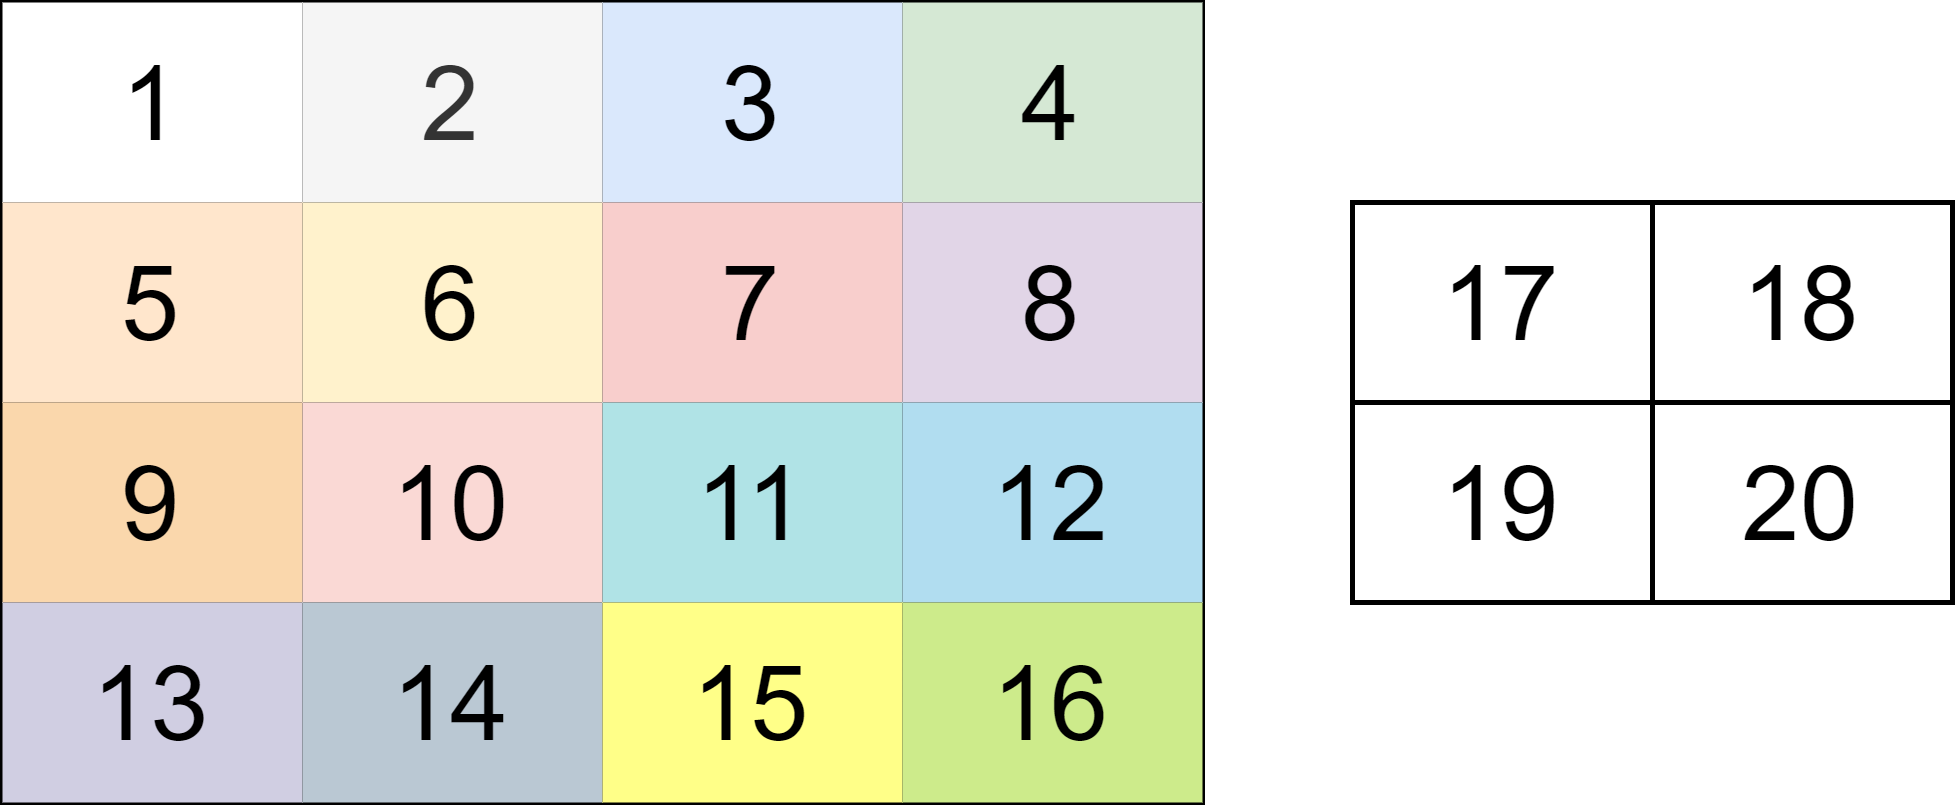
\includegraphics[width=4cm]{new_unrolling.png}
        \caption{Input image and weight}
        \label{input image and weight}
    \end{figure}

    Figure \ref{input image and weight} shows a mini-convolution,
    where exists a $1\times 4\times 4$ input image $X$  and a $1\times 2\times 2$ weight tensor $W$.
    For the sake of observation, each element of image is marked with different color and number.

    \begin{figure}[htbp]
        \centering
        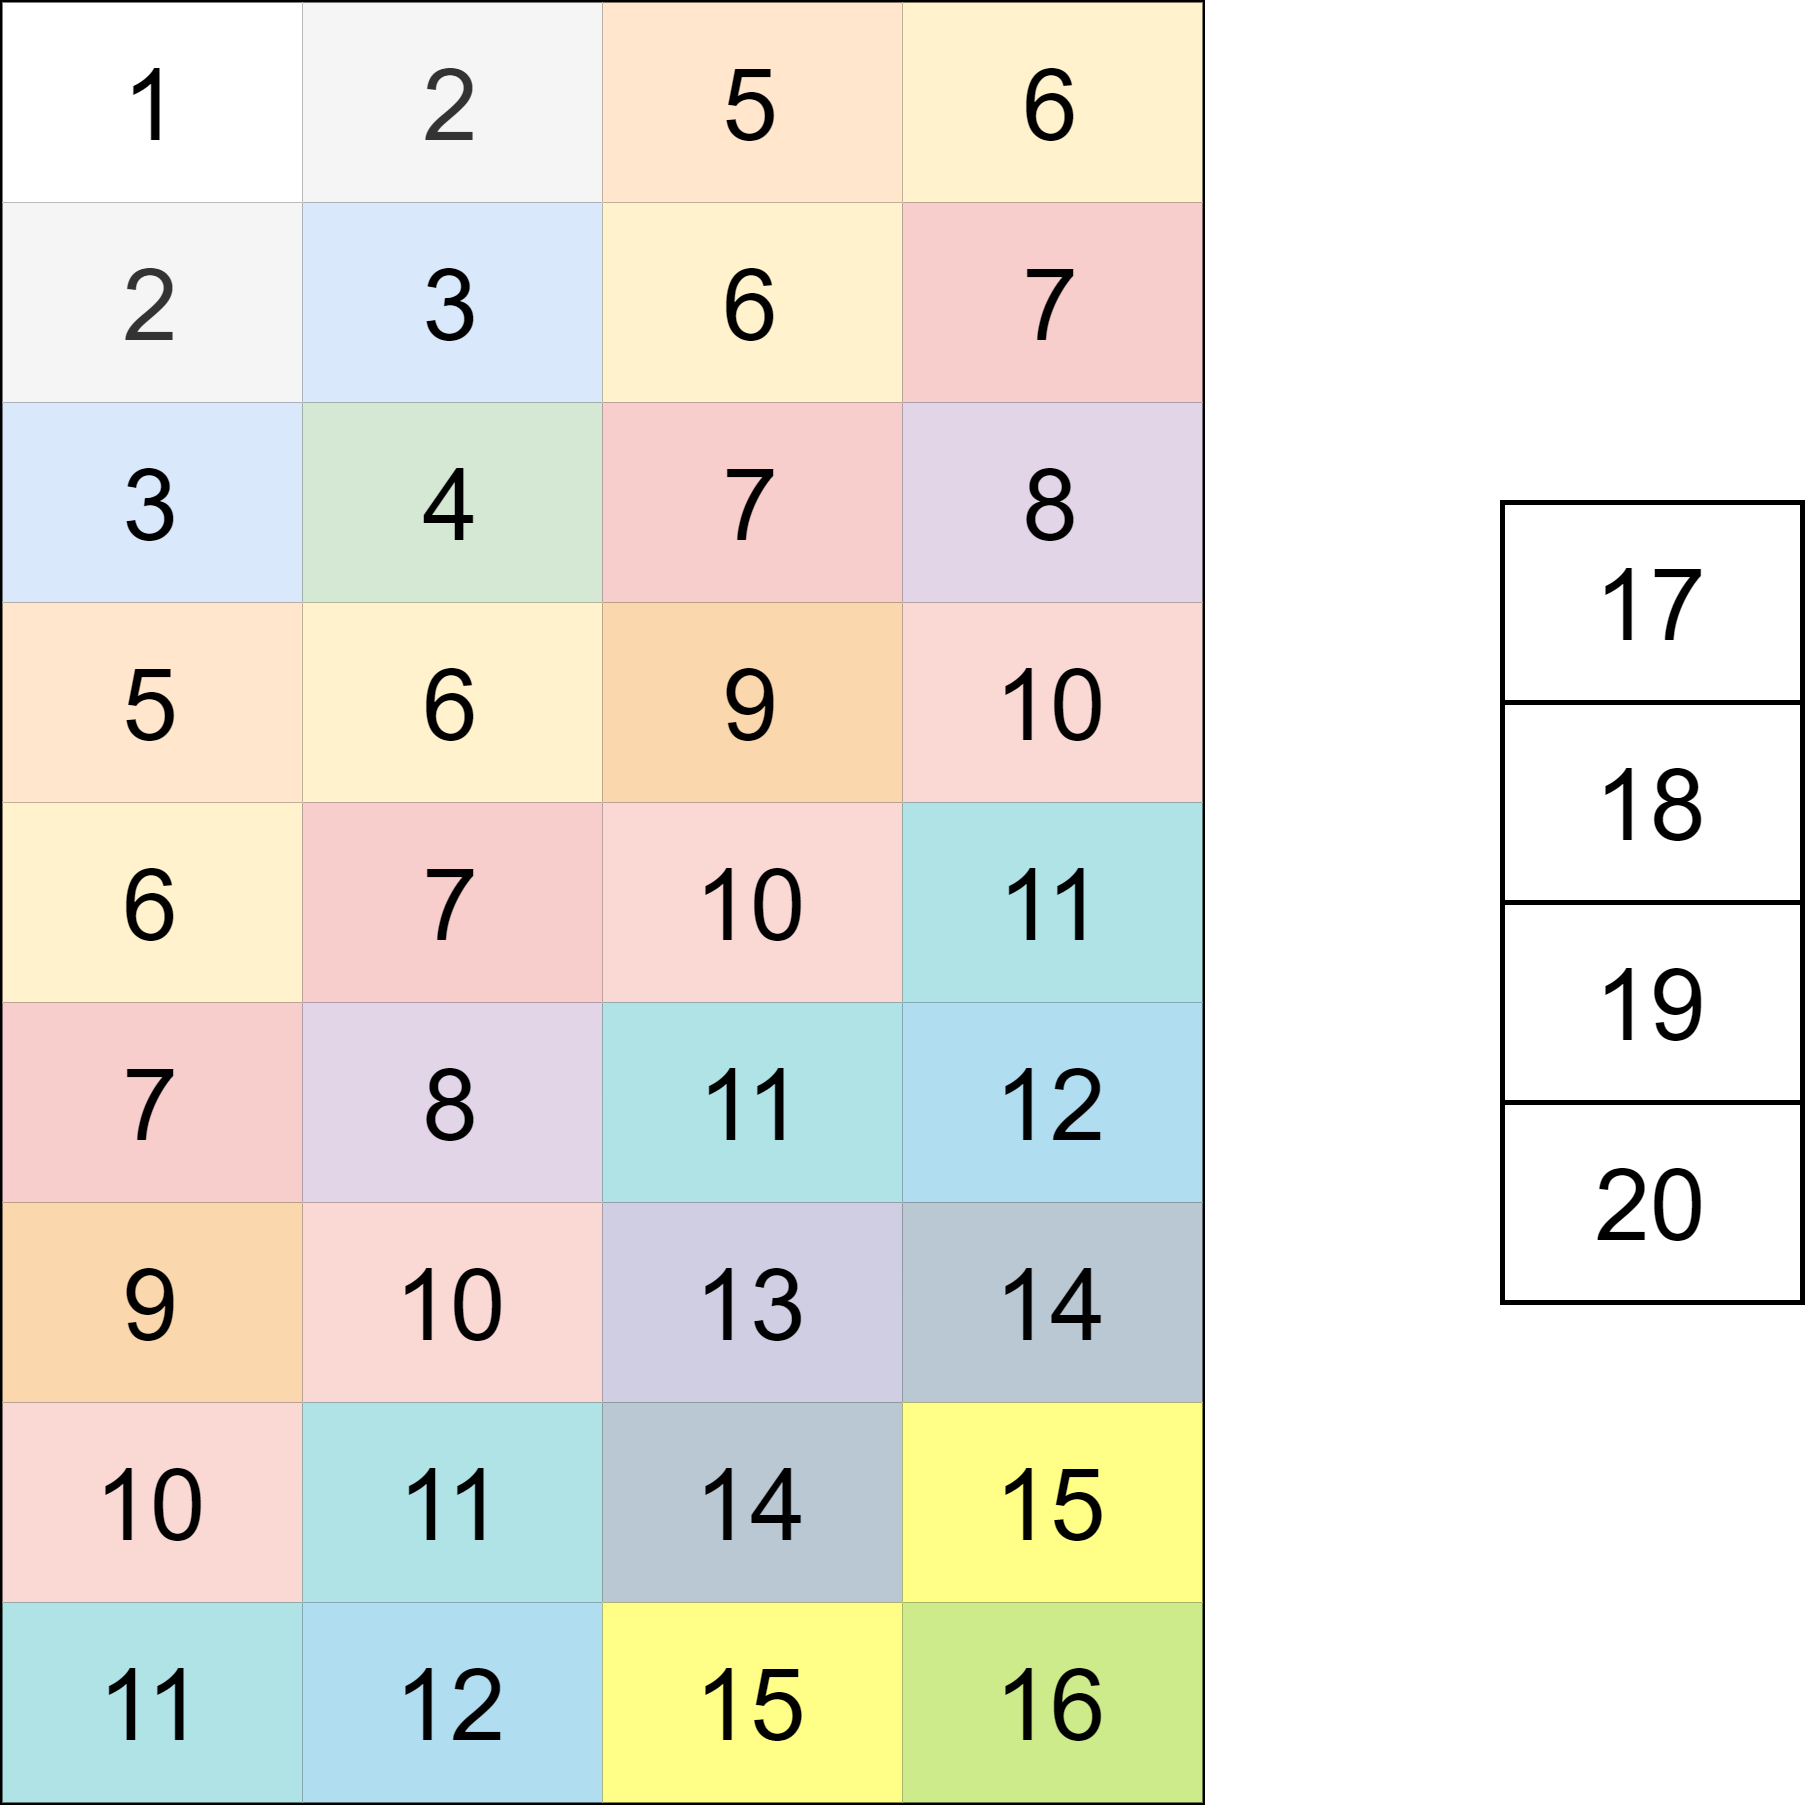
\includegraphics[width=4cm]{new_unrolling2.png}
        \caption{Rearranged image and weight}
        \label{rearrangement of image and weight}
    \end{figure}

    After rearrangement, matrix $(X',W')=Unroll(X,W)$
    is shown in Figure \ref{rearrangement of image and weight}.
    Elements that are not at the edge of the matrix repeated four times (such as NO.6)
    and some other elements were also duplicated.
    Since using the same random number to blind the duplicated element
    is more efficient so two parties can blind $(X,W)$ and
    construct the blinded $(X',W')$ locally instead of blinding $(X',W')$ directly.


    We propose an optimization of 2PC-convolution,
    that the communication consumption is reduced by
    not transmitting the duplicated elements.

    \textbf{Protocol procedure}:
    \begin{itemize}
        \item \textbf{1.} $TTP$ randomly chooses matrix $(A,B)$ of the same size of the original feature $X$ and filter weight $W$.
        \item \textbf{2.} $TTP$ evaluates $( A',B')=Unroll(A,B)$ and $C' =A'\cdot B' $.
        Then, $TTP$ sends $(\langle A\rangle ^{i},\langle B\rangle ^{i},\langle C'\rangle ^{i})$ to $\mathcal{P}_{i}$.
        \item \textbf{3.} $\mathcal{P}_{i}$ sets $\langle E\rangle ^{i}=\langle X\rangle ^{i}-\langle A\rangle ^{i}$
        and $\langle F\rangle ^{i}=\langle W\rangle ^{i}-\langle B\rangle ^{i}$
        and transmits $(\langle E\rangle ^{i},\langle F\rangle ^{i})$ to $\mathcal{P}_{1-i}$.
        \item \textbf{4.} $\mathcal{P}_{i}$ reconstruct $E = \langle E\rangle ^{0}+\langle E\rangle ^{1}$ and $F = \langle F\rangle ^{0}+\langle F\rangle ^{1}$
        and evaluates $(E',F')=Unroll(E,F)$ and $(A',B')=Unroll(A,B)$.
        \item \textbf{5.} $\mathcal{P}_{i}$ sets $\langle Z\rangle^{i}=i\cdot E' \cdot F' + \langle A'\rangle^{i} \cdot F' + E' \cdot \langle B'\rangle^{i} + \langle C'\rangle^{i}$.

    \end{itemize}

    % Essentially,
    By this way, communication overhead can be observably reduced to almost $ \frac{1}{width^{2}} $ of the original,
    where $width$ is the width of filter.
    % \section{Theoretical analysis}


    \subsubsection{Pooling layer}


    There are two types of pooling layer: average pooling and maximum pooling,
    which output the average or the maximum of $n\times n$ size submatrices respectively
    to construct the input image of next layer.
    We take $2\times 2$ window as an example to show how $\mathcal{P}_{0}$ and $\mathcal{P}_{1}$ compute the output of a submatrix.
    For each $2\times 2$ submatrix $X$, average pooling outputs $y_{avg}=\frac{X_{00}+ X_{01}+ X_{10}+  X_{11}}{4}$
    and max pooling outputs $y_{max}=max(X_{00}, X_{01}, X_{10},  X_{11})$
    $$  \langle X\rangle ^{0}= \begin{bmatrix}
        \langle X_{00}\rangle ^{0}& \langle X_{01}\rangle ^{0} \\
        \langle X_{10}\rangle ^{0}& \langle X_{11}\rangle ^{0}
       \end{bmatrix}\langle X\rangle ^{1}=\begin{bmatrix}
        \langle X_{00}\rangle ^{1}& \langle X_{01}\rangle ^{1} \\
        \langle X_{10}\rangle ^{1}& \langle X_{11}\rangle ^{1}
       \end{bmatrix}$$


    % Generally, we denote the calculation of pooling layer by $\langle Y\rangle = \langle Pooling(X)\rangle$.

    2PC-average pooling is easy to implement by locally division.
    To get the average of elements in submatrix $X$,
    $\mathcal{P}_{0}$ sets $\langle y_{avg}\rangle^{0} =$$ \frac{\langle X_{00}\rangle ^{0}+ \langle X_{01}\rangle ^{0}+
    \langle X_{10}\rangle ^{0}+ \langle X_{11}\rangle ^{0}}{4}$ and
    $\mathcal{P}_{1}$ sets $\langle y_{avg}\rangle^{1} = \frac{\langle X_{00}\rangle ^{1}+ \langle X_{01}\rangle ^{1}+
    \langle X_{10}\rangle ^{1}+ \langle X_{11}\rangle ^{1}}{4}$. This process can be done without interaction.

    2PC-maximum pooling layer can be computed via $\mathtt{comparison}$ protocol for
    $y_{max}=max(X_{00}, X_{01}, X_{10}, X_{11})$.
    The approach to compute this has been briefly discussed before and now we give it in detail.
    Consider that
    \begin{align*}
        &\enspace \enspace \enspace  max(X_{00}, X_{01}, X_{10}, X_{11}) \\
        &= max(X_{00},max(X_{01}, X_{10}, X_{11})) \\
      &= max(X_{00},max(X_{01},max(X_{10}, X_{11})))
    \end{align*}
    So the maximum of each submatrix can be obtained by running
    maximum protocol for three times.
    After repeating this process to each submatrix, parties can get the output matrix of the pooling layer.


    \subsubsection{Activation function}
    Here we explore one  activation functions: $ReLU()$, a typical continuous piecewise function.
    % which can be calculated referring to piecewise function protocol in 3.4.
    $$ReLU(x)=\begin{cases}
        0 & \text{ if } x \leqslant 0  \\
        x & \text{ if } x > 0
        \end{cases}$$
    $ReLU$ function has three dividing points: $dp_{0}= -\infty ,dp_{1}= 0, dp_{n}=+\infty$ and two sub-functions:
    $f_{1}(x)= 0 ,f_{2}(x)= x$.
    With $v_{j} = (1-sign(dp_{j-1}-x)\cdot sign(dp_{j}-x))/2$, this function can be represented as
    % $$ReLU(x)=\sum_{j=1}^{2}v_{j}\cdot f_{j}(x)=v_{1}\cdot f_{1}(x)+v_{2}\cdot f_{2}(x)=v_{1}\cdot 0 +v_{2}\cdot x=v_{2}\cdot x$$
    \begin{align*}
        ReLU(x)&=\sum_{j=1}^{2}v_{j}\cdot f_{j}(x)=v_{1}\cdot f_{1}(x)+v_{2}\cdot f_{2}(x)\\
        &=v_{1}\cdot 0 +v_{2}\cdot x\\
        &=v_{2}\cdot x\\
        &=\frac{(1-sign(dp_{1}-x)\cdot sign(dp_{2}-x))\cdot x}{2} \\
        &=\frac{(1-sign(0-x)\cdot sign(+\infty -x))\cdot x}{2} \\
        &=\frac{(1+sign(x))\cdot x}{2}
    \end{align*}

    Parties can follow $\mathtt{multiplication}$ protocol and $\mathtt{comparison}$ protocol to compute
    $\langle y\rangle=\langle ReLU(\langle x\rangle)\rangle=\frac{(1+\langle sign(\langle x\rangle)\rangle)\otimes \langle x\rangle}{2}$.



    \section{Theoretical Analysis}
    \begin{table}[!ht]

        \center
        \resizebox{0.45\textwidth}{!}{
        \begin{tabular}{|c|c|c|c|}\hline

           &computation(asymmetric)& communication(bits) & rounds     \\ \hline
        ABY&                   18$l$& $7l\cdot \kappa+(l^{2}+l)/2$ &6\\\hline
        Sharemind&               0&     3$l$               &$l$\\\hline
        2PC-NNP&                   0&   3                  &3 \\\hline
        \end{tabular}}
        \caption{Overhead of different 2PC-comparison schemes for a $l$-bits value }
        \label{Overhead of methods}
    \end{table}
    The biggest advantage of 2PC-NNP is that we design a novel $\mathtt{comparison}$ protocol which has
    a huge improvement over the previous work.
    We list the state-of-art 2PC-$\mathtt{comparison}$ protocol:
    ABY and Sharemind, and compare them to our work.
    As shown in Table \ref{Overhead of methods}, asymmetric encryption computation, communication bits and
    interaction rounds are listed.
    Obliviously, our scheme shows the best performance.4


    \section{Experiment}
    To evaluate the performance of our work, we conduct simulation experiment on a desktop (CPU: AMD Ryzen 7 5800H with 3.20GHz).
    We use two independent folders placed on different physical hard drives to simulate the two servers belonging to the
    data owner and the model provider for measuring the time cost of computation
    and we calculate the communication consumption by counting all of floating point numbers needed to be passed.
    We use Python 3.9.7 to implement our system and use some functions in the SPDZ library.
    All operations involved in the experiments are floating point operations.
    Files are written in form of npy format supported by Python, where a floating point number occupies about 0.0078Kb.
    For accurate and stable measurement, file transfer rate between servers is fixed at 10M/s.
    Each experiment was repeated 10 times.

    The experiments is divided into three parts: 1.basic operations 2.neural network layers 3.neural network implementation.

    % Computation time cost is directly measured by time functions provided by Python and the c
    % Since our system is an IO-intensive system, CPU shows better performance than GPU in file reading and writing.
    \subsection{Operations}


    \begin{figure}[htbp]
        \subfigure[multiplication] %第一张子图
        {
            \begin{minipage}{0.45\linewidth}
                \centering
                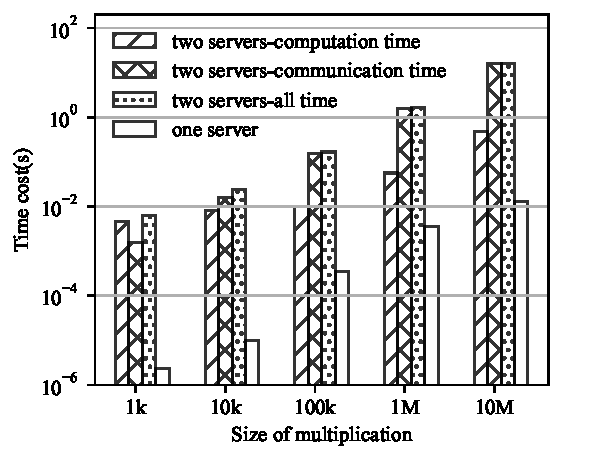
\includegraphics[width=4cm]{operation_mul.pdf}
                % \caption{operation mul}
                \label{operation_mul}
            \end{minipage}
        }
        \subfigure[matrix multiplication] %第二张子图
        {
            \begin{minipage}{0.45\linewidth}
                \centering
                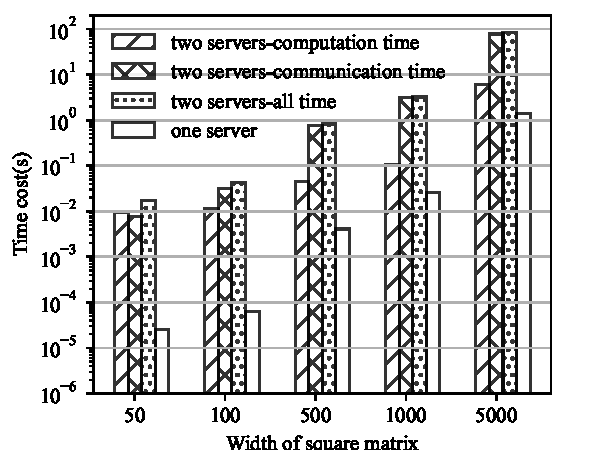
\includegraphics[width=4cm]{operation_matrix_mul.pdf}
                % \caption{operation matrix mul}
                \label{operation_matrix_mul}
            \end{minipage}
        }
        \caption{Experiment I-Overhead of 2PC-multiplication and matrix multiplication}
        \label{multiplication and matrix multiplication}

    \end{figure}

    \begin{figure}[htbp]

        \centering
        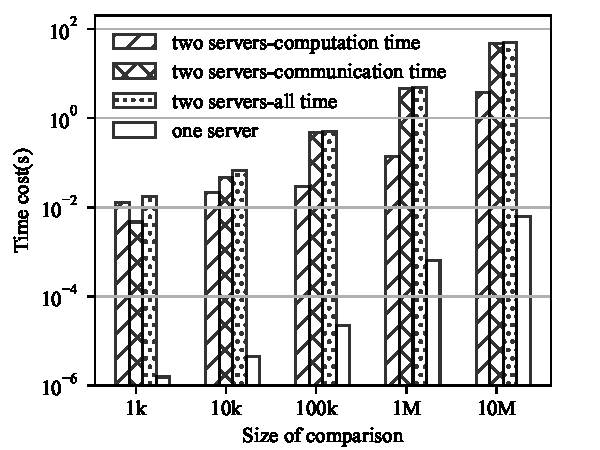
\includegraphics[width=5cm]{operation_compare.pdf}
        \caption{Experiment I-Overhead of 2PC-comparison}
        \label{operation_compare}
    \end{figure}
    In Experiment I, time consumption of basic operations including multiplication, comparison and matrix multiplication are measured.
    % Experiment results of multiplication and matrix multiplication are shown in \ref{operation_mul}
    In addition, we give the time consumption of one server operating directly as a reference.
    The data obtained is shown in Figure \ref{multiplication and matrix multiplication} and Figure \ref{operation_compare}.

    The time cost of secure two-party calculation is divided into two parts:
    local calculation and online communication.
    the time consumption of online communication increases linearly with the increase of the number of elements,
    while local computation time is more complicated.
    Due to the large number of writing and reading operations involved,
    there will be a lot of fixed time consumption for calling system file functions.

    The three operations show the same trend that
    When the number of elements achieves 10k and more,
    the communication time becomes longer than the calculation time
    which accounts for a substantial part of total time.
    Take matrix multiplication as an example,
    when the width is $1000$, the communication costs $3.12$s, accounting for $96\%$ of total time.

    \subsection{Neural network layers}
    In Experiment II, overhead of neural network layers including
    convolution layer, pooling layer and ReLU function are measured.



    \begin{table}[!ht]

        \center
        \resizebox{0.45\textwidth}{!}{
        \begin{tabular}{|c|c|c|c|c|c|}\hline

        \multicolumn{6}{|c|}{Convolution Layer}\\ \hline
        \multirow{2}{*}{feature size}&\multirow{2}{*}{size of filter}& \multicolumn{3}{c|}{cost time(s)}&communication \\

        \cline{3-5}
        \multirow{2}{*}{ }&\multirow{2}{*}{ }&computation&communication&all&size(Mb)  \\ \hline
        (64,56,56)& (64,64,3,3) & 0.64  & 0.18 & 0.82 &0.28\\ \hline
        (256,28,28)& (512,256,1,1) & 0.48 & 0.26 & 0.74 & 0.16 \\ \hline
        (256,14,14)& (256,256,3,3) & 0.20 & 0.50 & 0.70 & 0.096\\ \hline
        (1024,7,7)& (2048,1024,1,1) & 0.21 & 1.68 & 1.89 & 0.086 \\ \hline \hline




        \multicolumn{6}{|c|}{Pooling Layer}\\ \hline
        \multicolumn{2}{|c|}{\multirow{2}{*}{feature size}}& \multicolumn{3}{c|}{cost time(s)}&communication   \\

        \cline{3-5}
        \multicolumn{2}{|c|}{}&computation&communication&all&size(Mb)\\ \hline
        \multicolumn{2}{|c|}{(256,14,14)} & 0.088  & 0.26 & 0.35 &2.6	\\ \hline
        \multicolumn{2}{|c|}{(256,28,28)} & 0.107 & 1.05 & 1.16 & 10.5 \\ \hline
        \multicolumn{2}{|c|}{(256,56,56)} & 0.240  & 4.23 & 4.47 &42.3	\\ \hline
        \multicolumn{2}{|c|}{(256,112,112)} & 0.746 & 16.93 & 17.68 & 169.3 \\ \hline          \hline




        \multicolumn{6}{|c|}{ReLU}\\ \hline
        \multicolumn{2}{|c|}{\multirow{2}{*}{feature size}}& \multicolumn{3}{c|}{cost time(s)}&communication   \\


        % \multirow{2}{*}{\multicolumn{2}{c|}{feature size}}& \multicolumn{3}{c|}{time(s)}&communication   \\

        \cline{3-5}
        \multicolumn{2}{|c|}{} &computation&communication&all&size(Mb)\\ \hline
        \multicolumn{2}{|c|}{(256,14,14)} & 0.025  & 0.27 & 0.29 &2.7	\\ \hline
        \multicolumn{2}{|c|}{(256,28,28)} & 0.054 & 1.09 & 1.15 & 10.9 \\ \hline
        \multicolumn{2}{|c|}{(256,56,56)} & 0.160  & 4.39 & 4.55 &43.9	\\ \hline
        \multicolumn{2}{|c|}{(256,112,112)} & 0.631 & 17.56 & 18.19 & 175.6 \\ \hline

        \end{tabular}}

        \caption{Experiment II-Layers consumption}
        \label{Layers_consumption}
    \end{table}


    For different neural network layers,
    we select several representative shapes of features and filters
    to test the time cost.
    The result is shown in Table \ref{Layers_consumption}.
    In general, the computational overhead of neural network layers has been reduced to an acceptable range
    and the communication cost still account for the vast majority.




    \subsection{Neural Networks}
    To demonstrate the performance of our method in practice, we conduct
    time-consuming tests on a small network Lenet-5 \cite{Lenet5} and a large network Resnet50\cite{DeepResidualLearning}.
    The MNIST dataset, consisting of about 70000 images of size $1\times 28 \times 28$ with $10$ classes
    for handwriting recognition is used for training neural network models.
    Since the size of input image of Resnet50 is $3\times 224 \times 224$,
    we resize each image of MNIST dataset to $3\times 224 \times 224$ for training the Resnet50 model.
    Notably, we remove the batch normalization layers of Resnet50 because 2PC-NNP
    cannot implement the division of which the dividsor is a secret variable.


    \begin{table}[!ht]

        \center
        \resizebox{0.45\textwidth}{!}{
        \begin{tabular}{|c|c|c|c|c|}\hline
        \multirow{2}{*}{model}& \multicolumn{3}{c|}{time(s)}&communication  \\

        \cline{2-4}
        \multirow{2}{*}{ }&computation&communication&all&size(Mb) \\ \hline
        Lenet-5 & 0.375  & 0.32 & 0.69 &3.2	\\ \hline
        Resnet50 & 23.85 & 100.13 & 123.98 & 1001.3 \\ \hline
        \end{tabular}}
        \caption{Experiment III-Neural networks consumption}
        \label{neural networks consumption}
    \end{table}

    As shown in Table \ref{neural networks consumption}, 2PC-NNP shows an excellent performance
    both in medium and large neural networks. To evaluate the Resnet50,
    it costs 23.85s for computation and 100.13s for communication.

    \section{Conclusion and Future Work}
    In this work, we presented 2PC-NNP, a two-party computation framework for neural network predictions.
    This framework based on a novel 2PC-$\mathtt{comparison}$ protocol which does not involve asymmetric encryption operations.
    The 2PC-$\mathtt{comparison}$ protocol enables us to build a efficient framework neural network predictions.
    Furthermore, we design methods to evaluate each layer in neural network and implement an experiment on Resnet50 \cite{DeepResidualLearning}.
    This framework has great potential since we only consider the serial implementation of protocols.
    However, some computation can be excuted in parallel to reduce the rounds of interaction.
    This task can be considered in future work.
    \section{Appendix}
    Formalized protocols are presented here.

    \begin{figure}
        % \centering{\bf Two-party secure computation protocol for operations}
        \resizebox{0.5\textwidth}{!}{
        \begin{tabular}{lcl}
            \hline
            \multicolumn{3}{c}{\underline{$\mathtt{Multiplication}$}:}\\
            \multicolumn{3}{l}{\textbf{Target}: compute $\langle z\rangle  = \langle x\rangle  \otimes \langle y\rangle $}\\
            % \textbf{Target}: compute $\langle z\rangle  = \langle x\rangle  \cdot \langle y\rangle $\\
            \textbf{Input}:\\
            % & \hfil\underline{$\mathtt{Multiplication}$}:\hfil\\
            $\mathcal{P}_{0}$ &  &  $\mathcal{P}_{1}$ \\
            $\{(\langle x\rangle ^{0} , \langle y\rangle ^{0})$,
            &
            &
            $\{(\langle x\rangle ^{1} , \langle y\rangle ^{1})$,

            \\

            mul-triple:$
            (\langle a\rangle ^{0},\langle b\rangle ^{0},\langle c\rangle ^{0})\}$
            &
            &
            mul-triple:$ (\langle a\rangle ^{1},\langle b\rangle ^{1},\langle c\rangle ^{1})\}$
            \\
            \textbf{Procedure}:\\
            $\mathcal{P}_{0}$ &  &  $\mathcal{P}_{1}$ \\
            $\langle e\rangle ^{0}\leftarrow\langle x\rangle ^{0}-\langle a\rangle ^{0}$
            &
            &
            $\langle e\rangle ^{1}\leftarrow\langle x\rangle ^{1}-\langle a\rangle ^{1}$
            \\
            $\langle f\rangle ^{0}\leftarrow\langle y\rangle ^{0}-\langle b\rangle ^{0}$
            &
            &
            $\langle f\rangle ^{1}\leftarrow\langle y\rangle ^{1}-\langle b\rangle ^{1}$
            \\
            & $\underrightarrow{~~~~~~(\langle e\rangle ^{0},\langle f\rangle ^{0})~~~~~~}$ &\\
            & $\underleftarrow{~~~~~~(\langle e\rangle ^{1},\langle f\rangle ^{1})~~~~~~}$ &\\
            $e\leftarrow\langle e\rangle ^{0}+\langle e\rangle ^{1}$& &$e\leftarrow\langle e\rangle ^{0}+\langle e\rangle ^{1}$\\
            $f\leftarrow\langle f\rangle ^{0}+\langle f\rangle ^{1}$& &$f\leftarrow\langle f\rangle ^{0}+\langle f\rangle ^{1}$\\
            $\langle z\rangle^{0}\leftarrow f\cdot \langle a\rangle^{0}$
            & &
            $\langle z\rangle^{1}\leftarrow e \cdot f + f\cdot \langle a\rangle^{1}$\\
            $+e \cdot \langle b\rangle^{0} + \langle c\rangle^{0}$& &$+e \cdot \langle b\rangle^{1} + \langle c\rangle^{1}$\\
            \hline




        \end{tabular}}

    \end{figure}
    \begin{figure}

        \centering%{\bf Two-party secure computation protocol for operations}
        \resizebox{0.5\textwidth}{!}{
        \begin{tabular}{lcl}
            \hline
            \multicolumn{3}{c}{\underline{$\mathtt{Comparison}$}:}\\
            \textbf{Computation for $sign(x)$}:&&\\
            \textbf{Target}: compute $\langle s\rangle  = \langle sign(\langle x \rangle )\rangle $\\
            \textbf{Input}:\\
            % & \hfil\underline{$\mathtt{Multiplication}$}:\hfil\\
            $\mathcal{P}_{0}$ &  &  $\mathcal{P}_{1}$ \\
            $\{\langle x\rangle ^{0}$,
            &
            &
            $\{\langle x\rangle ^{1}$,

            \\

            comp-triple:$
            (\langle u\rangle ^{0},\llbracket u \rrbracket ^{0})\}$
            &
            &
            comp-triple:$ (\langle u\rangle ^{1},\llbracket u \rrbracket ^{1})\}$\\
            \textbf{Procedure}:\\
            $\mathcal{P}_{0}$ &  &  $\mathcal{P}_{1}$ \\
            % \multicolumn{3}{c}{$\underleftrightarrow{~~~\text{compute }
            % \langle z\rangle = \langle u\rangle \cdot \langle x\rangle }~~~$}\\
            \hdashline
            \multicolumn{3}{c}{run $\mathtt{multiplication}$ protocol to}\\
            \multicolumn{3}{c}{$\text{compute }
            \langle z\rangle = \langle u\rangle \otimes \langle x\rangle $ }\\
            gets $\langle z\rangle ^{0}$& &gets $\langle z\rangle ^{1}$\\

            \hdashline
            % & $\underrightarrow{~~~~~~~\langle z\rangle ^{0}~~~~~~~}$~~~~~~ &\\
            & $\underleftarrow{~~~~~~~\langle z\rangle ^{1}~~~~~~~}$~~~~~~ &\\
            $z\leftarrow\langle z\rangle ^{0}+\langle z\rangle ^{1}$& &\\
            % if $z = 0$:& &if $z = 0$:\\
            % ~~~$\langle s\rangle ^{0}\leftarrow 0$& &~~~$\langle s\rangle ^{1}\leftarrow 0$\\
            % ~~~\textbf{Finish protocol} & &~~~\textbf{Finish protocol}\\
            % else:& &else:\\
            % ~~~\textbf{Continue} & &~~~\textbf{Continue}\\
            $\llbracket s \rrbracket^{0}
            \leftarrow sign(\frac{1}{\llbracket u \rrbracket^{0}})$&
            &$\llbracket s \rrbracket^{1}
            \leftarrow sign(\frac{z}{\llbracket u \rrbracket^{1}})$\\

            \hdashline
            \multicolumn{3}{c}{run $\mathtt{multiplication}$ protocol to}\\
            \multicolumn{3}{c}{compute $
            \langle s\rangle = \llbracket s \rrbracket ^{0} \otimes \llbracket s \rrbracket ^{1}$}\\

            gets $\langle s\rangle ^{0}$& &gets $\langle s\rangle ^{1}$\\

            % \multicolumn{3}{c}{on input $(\mathcal{P}_{0}:(\llbracket s \rrbracket ^{0},0),\mathcal{P}_{1}:(0,\llbracket s \rrbracket ^{1}))$ }\\
            \hdashline
            % $\langle s\rangle ^{0} \leftarrow \langle product\rangle^{0}$&&$\langle s\rangle ^{1} \leftarrow \langle product\rangle^{1}$\\
            \hline
        \end{tabular}}

    \end{figure}
    \begin{figure}
        \centering%{\bf Two-party secure computation protocol for operations}
        \resizebox{0.5\textwidth}{!}{
        \begin{tabular}{lcl}
            \hline
            \multicolumn{3}{l}{\textbf{Computation for $max(x)$}:}\\
            \multicolumn{3}{l}{\textbf{Target}: compute $\langle maximum\rangle  = \langle max(\langle x\rangle,\langle y\rangle)\rangle$}\\


            % \textbf{Target}: compute $\langle max\rangle  = \langle max(\langle x\rangle,\langle y\rangle)\rangle$\\
            \textbf{Input}:\\
            % & \hfil\underline{$\mathtt{Multiplication}$}:\hfil\\
            $\mathcal{P}_{0}$ &  &  $\mathcal{P}_{1}$ \\
            $\{\langle x\rangle ^{0} , \langle y\rangle ^{0}\}$
            &
            &
            $\{\langle x\rangle ^{1} , \langle y\rangle ^{1}\}$
            \\



            \textbf{Procedure}:\\
            $\mathcal{P}_{0}$ &  &  $\mathcal{P}_{1}$ \\
            % \multicolumn{3}{c}{$\underleftrightarrow{~~~\text{compute }
            % \langle z\rangle = \langle u\rangle \otimes \langle x\rangle }~~~$}\\
            $\langle \Delta\rangle ^{0} \leftarrow \langle x\rangle^{0}-\langle y\rangle^{0}$
            & ~~~~~~~~~~~~~~~~~~~~~~~~~~~~~~~~~~~~&
            $\langle \Delta\rangle ^{1} \leftarrow \langle x\rangle^{1}-\langle y\rangle^{1}$\\
            \hdashline
            \multicolumn{3}{c}{run $\mathtt{comparison}$ protocol to}\\
            \multicolumn{3}{c}{compute
            $\langle s\rangle=sign(\langle \Delta\rangle)$}\\
            gets $\langle s\rangle ^{0}$& &gets $\langle s\rangle ^{1}$\\

            \hdashline
            \hdashline
            \multicolumn{3}{c}{run $\mathtt{multiplication}$ protocol to}\\
            \multicolumn{3}{c}{compute
            $\langle maximum\rangle=\frac{(\langle s\rangle+1)\otimes \langle x\rangle+ (-\langle s\rangle+1)\otimes \langle y\rangle}{2}$}\\
            gets $\langle maximum\rangle ^{0}$& &gets $\langle maximum\rangle ^{1}$\\
            \hdashline
            \hline

        \end{tabular}}

    \end{figure}
    \begin{figure}
        \centering%{\bf Two-party secure computation protocol for operations}
        \resizebox{0.5\textwidth}{!}{
        \begin{tabular}{lcl}
            \hline
            \multicolumn{3}{l}{\textbf{Computation for piecewise function $F(x)$}:}\\
            \multicolumn{3}{l}{\textbf{Target}: compute $\langle value\rangle  = \langle F(\langle x\rangle)\rangle $}\\
            \textbf{Input}:\\
            % & \hfil\underline{$\mathtt{Multiplication}$}:\hfil\\
            $\mathcal{P}_{0}$ &~~~~~~~~~~~~~~~~~~~~~~~~~~~ &  $\mathcal{P}_{1}$ \\
            $\{\langle x\rangle ^{0} , F(),(dp_{0},...,dp_{n}),$
            &
            &
            $\{\langle x\rangle ^{1} ,  F(),(dp_{0},...,dp_{n}),$
            \\
            $(f_{0}(),...,f_{n}())\}$
            &
            &
            $(f_{0}(),...,f_{n}())\}$
            \\

            \textbf{Procedure}:\\
            $\mathcal{P}_{0}$ &  &  $\mathcal{P}_{1}$ \\
            \hdashline
            \multicolumn{3}{l}{\textbf{For} each $dp_{j},j\in\{1,2,...,n-1\}$:}\\
            \multicolumn{3}{c}{run $\mathtt{comparison}$ protocol to}\\
            \multicolumn{3}{c}{compute
            $\langle s_{j}\rangle=\langle sign(dp_{j}-\langle x\rangle)\rangle$}\\
            ~~~~~~~gets $\langle s_{j}\rangle ^{0}$& &~~~~~~~gets $\langle s_{j}\rangle ^{1}$\\
            \hdashline
            \hdashline
            \multicolumn{3}{l}{\textbf{For} each $v_{j},j\in\{1,2,...,n-1\}$:}\\

            \multicolumn{3}{c}{run $\mathtt{multiplication}$ protocol to}\\
            \multicolumn{3}{c}{compute
            $\langle v_{j} \rangle= \frac{1-\langle s_{j}\rangle\otimes \langle s_{j-1}\rangle}{2}$}\\
            ~~~~~~~gets $\langle v_{j}\rangle ^{0}$& &~~~~~~~gets $\langle v_{j}\rangle ^{1}$\\
            \hdashline
            \hdashline
            \multicolumn{3}{c}{run $\mathtt{multiplication}$ protocol to}\\
            \multicolumn{3}{c}{compute
            $\langle value\rangle=\langle F(\langle x\rangle)\rangle=\sum_{j=1}^{n}\langle v_{j}\rangle\otimes \langle f_{j}(\langle x\rangle)\rangle$}\\
            gets $\langle value\rangle ^{0}$& &gets $\langle value\rangle ^{1}$\\
            \hdashline
            % $\langle s\rangle ^{0} \leftarrow \langle value\rangle^{0}$&&$\langle s\rangle ^{1} \leftarrow \langle value\rangle^{1}$\\
            \hline

        \end{tabular}}

    \end{figure}








% Use \bibliography{yourbibfile} instead or the References section will not appear in your paper
\bibliography{aaai23}


\bibentry{ABY3}
\bibentry{ABY}
\bibentry{EfficientMultipartyProtocols}
\bibentry{ChironCloud}
\bibentry{HighPerformanceConvolutional}
\bibentry{ObliviousNeuralNetwork}
\bibentry{DeepResidualLearning}
\bibentry{MaliciouslySecureMatrixMultiplication}
\bibentry{CryptoNets}
\bibentry{Sharemind}
\bibentry{Homomorphic1}
\bibentry{Homomorphic2}
\bibentry{Lenet5}
% \bibentry{}
% \bibentry{}
% \bibentry{}
% \bibentry{}
% \bibentry{}
% \bibentry{}


\end{document}
